\documentclass[12pt]{article}

\usepackage{fontspec}
\usepackage{polyglossia}
\usepackage{geometry}
\usepackage{graphicx}

\usepackage{amsmath,
            amsthm,
            amssymb
}

\usepackage{unicode-math,
            tensor
}

\usepackage{wrapfig, 
            hyperref,
            multicol,
            multirow,
            tabularx,
            booktabs,
            makecell
}

\usepackage{}

\geometry{a4paper,
          total={170mm,255mm},
          left=10mm,
          top=15mm,
}

\setdefaultlanguage{russian}
\setotherlanguage{english}
\setkeys{russian}{babelshorthands=true}

\defaultfontfeatures{Ligatures=TeX}
\setmainfont{STIX Two Text}
\setmathfont{STIX Two Math}
\DeclareSymbolFont{letters}{\encodingdefault}{\rmdefault}{m}{it}

\newfontfamily{\cyrillicfont}{STIX Two Text} 
\newfontfamily{\cyrillicfontrm}{STIX Two Text}
\newfontfamily{\cyrillicfonttt}{Courier New}
\newfontfamily{\cyrillicfontsf}{STIX Two Text}

\renewcommand{\thefigure}{\thesection.\arabic{figure}}
\renewcommand{\thetable}{\thesection.\arabic{table}}
\numberwithin{equation}{section}

\renewcommand{\qedsymbol}{$\blacksquare$}
\theoremstyle{definition}
\newtheorem{definition}{Опр.}[section]
\theoremstyle{remark}
\newtheorem{statement}{Утв.}[section]
\theoremstyle{plain}
\newtheorem{theorem}{Теор.}[section]

\addto\captionsrussian{
  \renewcommand{\figurename}{Рис.}
  \renewcommand{\tablename}{Табл.}
  \renewcommand{\proofname}{Док-во}
}

\graphicspath{{./img/}}
\everymath{\displaystyle}

\newcommand{\RNumb}[1]{\uppercase\expandafter{\romannumeral#1\relax}}
\newcommand{\llabel}[1]{\label{\thesubsection:#1}}
\newcommand{\lref}[1]{\ref{\thesubsection:#1}}

\begin{document}

\paragraph{О-01}
Какова интенсивность света в центре дифракционной картины от круглого экрана, если он закрывает всю первую зону Френеля? Интенсивность света в отсутствие экрана равна $I_0$.\\

\begin{wrapfigure}[12]{r}{0.4\linewidth}
	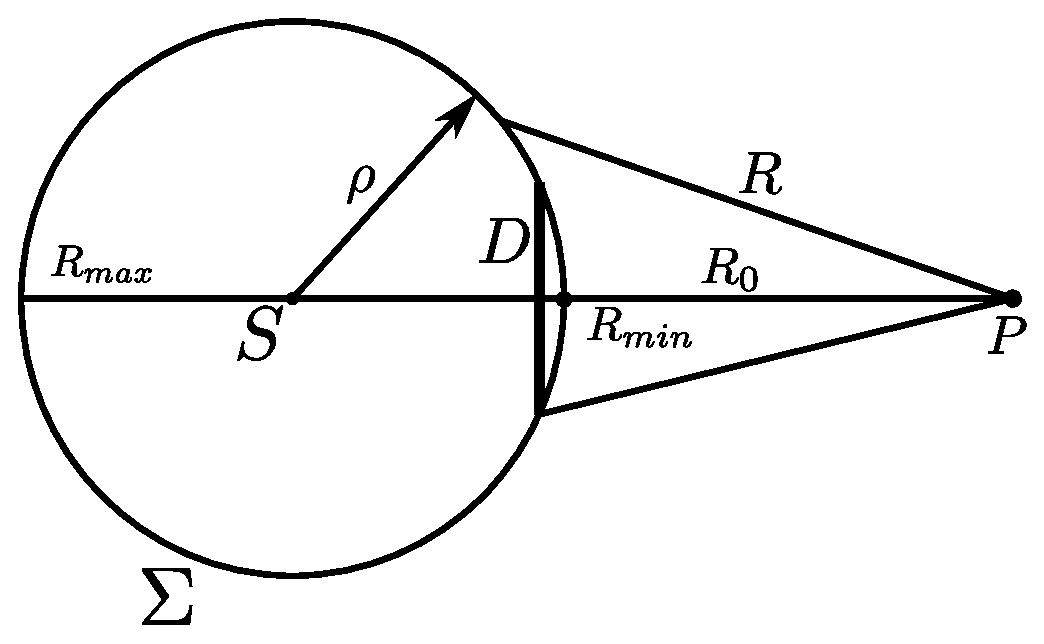
\includegraphics[width=1\linewidth]{img/o-01}
	\caption{Схема задачи}
	\label{o-01-diafrag}
\end{wrapfigure}

По формуле для напряженности электрического поля света, пропущенного через диафрагму радиуса $R_{max}$, и закрытой центральной областью радиуса $R_{max}$. (см. Рис. \ref{o-01-diafrag}) получим:
\begin{flalign}
\begin{split}
E &= E_0(K(R_{min})e^{ik(R_{min}-R_0)} - \\
  &- K(R_{max})e^{ik(R_{max}-R_0)}),
\end{split}
\label{o-01-formula}
\end{flalign}
где $K(R)$ - медленно монотонно убывающая функция такая, что $K(R_0) = 1$ и $K(R_0 + 2\rho) = 0$

Из того, что круглый экран закрывает первую зону Френеля получим 
$R_{max} = R_0 + 2\rho$, $\displaystyle R_{min} = R_0 + \frac{\lambda}{2}$, где $\lambda$ - длина волны света. Тогда $K(R_{max}) = 0$ и из (\ref{o-01-formula}):
\begin{flalign*}
&E = E_0K(R_0+\frac{\lambda}{2})e^{ik\lambda/2}
\Rightarrow (k = \frac{2\pi}{\lambda}) \\ \Rightarrow
&E = E_0K(R_0+\frac{\lambda}{2})e^{i\pi}
\Rightarrow (e^{i\pi} = -1, K(R_0 + \frac{\lambda}{2}) = K_1) \\ \Rightarrow
&E = -E_0K_1
\end{flalign*}
Тогда интенсивность света находится по формуле:
$$
I = E^2 \Rightarrow I = E_0^2K_1^2 = I_0K_1^2
$$
\end{document}